In \figref{fig:9.10.5.3.1} or,\figref{fig:9.10.5.3.2},$\angle PQR = 100\degree$,where $P,Q$ and $R$ are points on a circle with centre $O$.Find $\angle OPR$.

\textbf{Solution :}
\begin{table}[H]
    \centering
        \begin{tabular}{|c|c|c|}
    \hline
    \textbf{Input Parameters} &\textbf{Description} &\textbf{Value} \\
    \hline
     $\vec{O}$& Center(at origin)&$\vec{0}$\\
     \hline
 $r$ & Radius &1\\
 \hline
 $\theta$&$\angle PQR$&$100\degree$\\
 \hline
 $\theta_1$&$\angle NOQ $&$\theta_1\degree$\\
 \hline
 $\theta_2$&$\angle NOP $&$165\degree$\\
 \hline
 $\theta_3$&$\angle NOR $&$5\degree$\\
 \hline
  \end{tabular}

    \caption{Table of input parameters}
    \label{tab:9.10.5.3.1}
\end{table}

\begin{table}[H]
    \centering
        \begin{tabular}{|c|c|c|}
    \hline
        \textbf{Output Parameters} &\textbf{Description} &\textbf{Value} \\
\hline
          $\vec{Q}$ & Point &$\myvec{\cos{\theta_1}\\\sin{\theta_1}}$\\
          \hline
          $\vec{P}$ & Point &$\myvec{\cos{\theta_2}\\\sin{\theta_2}}$ \\
         \hline
          $\vec{R}$ & Point &$\myvec{\cos{\theta_3}\\sin{\theta_3}}$ \\
         \hline
    \end{tabular}

    \caption{Table of output parameters}
    \label{tab:9.10.5.3.2}
\end{table}

For getting the value of the $\angle NOQ$

\begin{align}
    \cos{\theta}&=\frac{\brak{\vec{R-Q}}^{\top}\brak{\vec{P-Q}}}{\vec{\norm{R-Q}\norm{P-Q}}}\\
    or,\cos{\theta}&=\frac{\sin{\frac{\theta_1+\theta_2}{2}}\cos{\frac{\theta_2+\theta_3}{2}}}{\sin{\frac{\theta_2-\theta_1}{2}}}\\
    so,\theta_1&=2\tan^{-1}\brak{\tan\brak{{\frac{\theta_2}{2}}}\brak{\frac{\cos{\theta}+\cos{\frac{\theta_2+\theta_3}{2}}}{\cos{\theta}-\cos{\frac{\theta_2+\theta_3}{2}}}}}\\
    \implies \theta_1&=136.696\degree\\
    or,\theta_1&=2\tan^{-1}\brak{\tan\brak{{\frac{\theta_2}{2}}}\brak{\frac{\cos{\theta}-\cos{\frac{\theta_2+\theta_3}{2}}}{\cos{\theta}+\cos{\frac{\theta_2+\theta_3}{2}}}}}\\
    \implies \theta_1&=175\degree\\
\end{align}
For getting the value of the $\angle OPR$
\begin{align}
    \angle OQP +\angle OQR &=\theta\\
    \angle QOR &=180-2\angle OQR,\brak{OQ=OR}\\
        \angle QOP &=180-2\angle OQP,\brak{OQ=OP}\\
        or,\angle POR &= 360-\brak{\angle QOP+\angle QOR}\\
        \implies \angle POR &= 2\brak{\angle OQP +\angle OQR}\\
        &=2\theta\\
    \angle POR +\angle ORP +\angle OPR &= 180\degree\\
    \angle POR +2\angle OPR&= 180\degree, \brak{OR=OP}\\
\angle OPR &= \frac{180\degree-2\theta}{2}\\
 \angle OPR &=-10\degree
 \end{align}


  \begin{figure}[H]                              
 \centering                          
 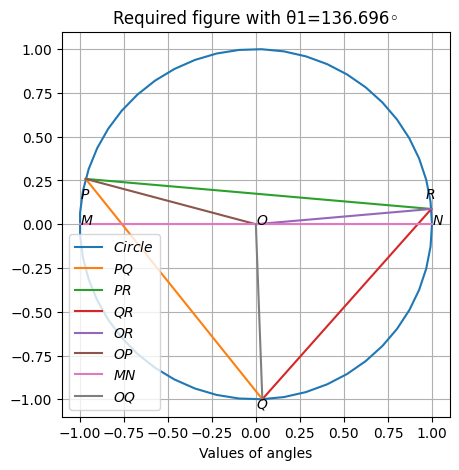
\includegraphics[width=\columnwidth]{chapters/9/10/5/3/fig/9.10.5.3.1.png}
\caption{}
	  \label{fig:9.10.5.3.1}
  \end{figure}
   \begin{figure}[H]                              
 \centering                          
 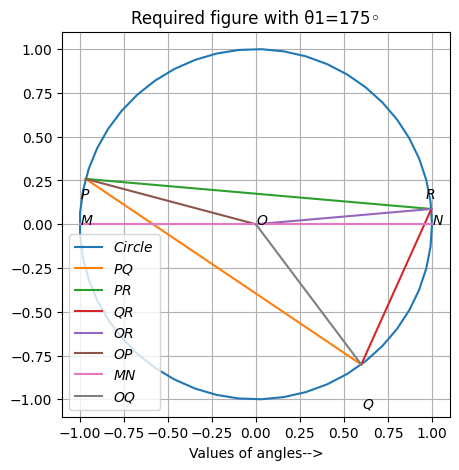
\includegraphics[width=\columnwidth]{chapters/9/10/5/3/fig/9.10.5.3.2.png}
\caption{}
	   \label{fig:9.10.5.3.2}
  \end{figure}
